\documentclass[10pt,twocolumn,letterpaper]{article}
\usepackage{cvpr}
\usepackage{graphicx}
\usepackage{booktabs}
\usepackage{multirow}
\usepackage{hyperref}

\title{MLPs, CNNs, Autoencoders, SVMs and Clustering on CIFAR-10}

\author{Manish Yadav\\
Roll number: p26ai0008\\
Repository: \texttt{https://github.com/manish-yadav/p26ai0008-ml-assignment3}\\
Final commit: \texttt{4796a15cb78994c88445f600f0b2cca01ecbcaa9}
}

\begin{document}
\maketitle

\begin{abstract}
This report answers the four questions of Assignment 3 on CIFAR-10.
For Q1 we separate two explanations for why plain MLPs underperform: missing translation invariance and insufficient capacity.
Pooling pixels before an MLP of matched size beats both a larger plain MLP and a smaller one, so the inductive bias matters more than parameters at this budget.
A 20\% wrong-label run shows clean examples are learned before noisy ones are memorised, with validation peaking at epoch 22 of 50.
For Q2 a CNN with a matched parameter budget reaches 69.9\% test accuracy versus 52.5\% for the MLP; a fixed pixel permutation costs the CNN 23.3 points but the MLP only 1.2, and retraining on grayscale closes part of the gap, supporting weight sharing over colour as the main cause.
For Q3 larger bottlenecks reconstruct better, but a denoising autoencoder (DAE) trained on Gaussian noise ($\sigma{=}0.25$) lifts classification of corrupted images from 31.4\% to 50.9\% and also carries more class information in linear probes (48.0\%) than the clean autoencoder with the best reconstruction (44.1\%).
For Q4, on a frozen 10{,}000-point subset of AE features, an RBF SVM at $C{=}10$ is selected on validation (48.6\%) and reaches 49.8\% test accuracy, while $k$-means on the same representation only reaches ARI 0.042 and purity 22.6\%, showing the clusters and the classes disagree.
\end{abstract}

\section{Common setup}
All experiments use CIFAR-10 with PyTorch, scikit-learn, NumPy and Matplotlib only.
No pretrained networks, external data, or automatic tuning are used.
The 50{,}000 training images are split once into 45{,}000 train and 5{,}000 validation images with \texttt{sklearn.train\_test\_split(stratify=y, random\_state=260008)}; the seed 260008 is the roll number digits \texttt{p26ai0008} read in order.
Both halves contain exactly 500 images per class on the validation side.
The split is stored in \texttt{split/cifar10\_split.npz} and reused by every script.
All classifiers train for 25 epochs with Adam, learning rate $10^{-3}$, batch size 128, cross-entropy loss, and fixed torch seed 260008.
Model selection uses validation accuracy only.
The official 10{,}000-image test set is evaluated exactly once per final model, at the end of training, and never used for any choice; the Q1b memorisation model never touches the test set.
Every run writes a per-epoch CSV log and a JSON result; all numbers in this report come from these files.
Pixel values are scaled to $[0,1]$.

\section{Q1: why MLPs perform poorly}
\subsection{Comparison design (Q1a)}
We take \emph{no built-in spatial invariance} as the main reason a plain MLP struggles on CIFAR-10: each weight sees one fixed pixel, so the network must relearn shifted versions of the same pattern.
A rival explanation is \emph{insufficient capacity}: 3072 inputs may simply need more units.
We separate the two with four models trained under an identical budget (same epochs, optimiser, learning rate, batch size, seed):
\begin{itemize}\itemsep1pt
\item \textbf{MLP-S}: $3072{\to}128{\to}128{\to}10$, 0.41M parameters (capacity axis).
\item \textbf{MLP-L}: $3072{\to}500{\to}500{\to}10$, 1.79M parameters (reference).
\item \textbf{MLP-B}: MLP-L trained with random $\pm4$-pixel shifts per batch (invariance through data).
\item \textbf{MLP-P}: MLP-L architecture on $2{\times}2$ average-pooled inputs (768 dims), 1.78M parameters (invariance through architecture).
\end{itemize}
The comparison is fair in the sense fixed before running: identical training budget, and the three 1.78--1.79M models differ by at most 0.7\% in parameters, so MLP-P is not simply bigger.
Averaging $2{\times}2$ blocks discards precise pixel position, which is the bias a convolution shares, but keeps a fixed, non-local receptive field, so MLP-P is still a pure MLP.

\begin{table}[t]
\centering\small
\begin{tabular}{lccccc}
\toprule
Model & Input & Params & Train & Val & Test \\
\midrule
MLP-S & 3072 & 0.41M & 56.8 & 51.7 & 51.2 \\
MLP-L & 3072 & 1.79M & 64.4 & 51.5 & 52.5 \\
MLP-B & 3072, shift aug. & 1.79M & 49.3 & 51.0 & 49.4 \\
MLP-P & 768 pooled & 1.78M & 69.4 & 54.2 & \textbf{53.9} \\
\bottomrule
\end{tabular}
\caption{Q1a after 25 epochs. Train accuracy is on clean images for MLP-S/L/P and on the shifted training views for MLP-B.}
\label{tab:q1a}
\end{table}

\begin{figure}[t]
\centering
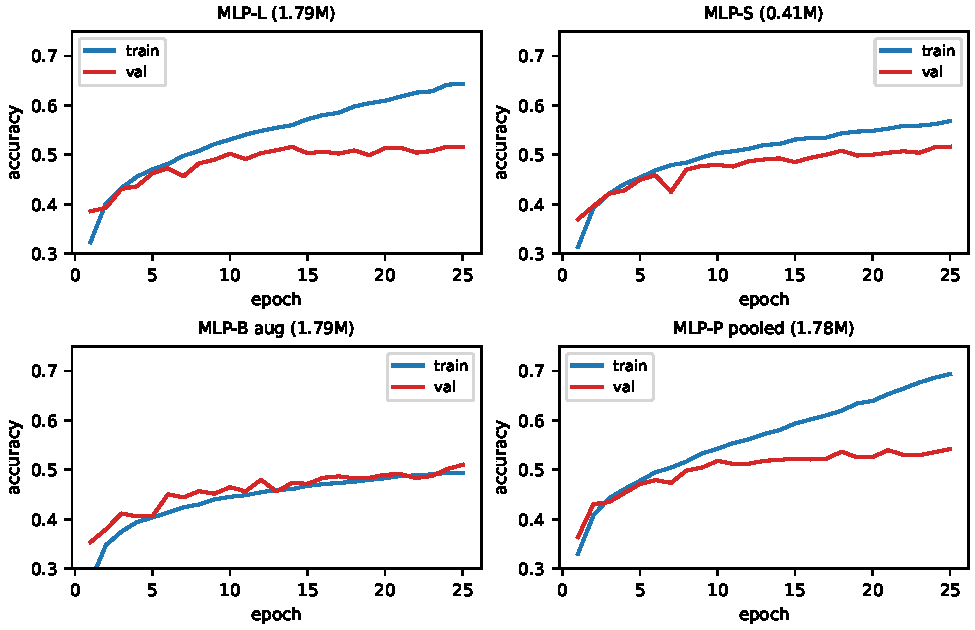
\includegraphics[width=\linewidth]{../figures/q1a_curves.pdf}
\caption{Q1a training and validation curves. Validation differences between the three 1.79M models stay small; MLP-P generalises best.}
\label{fig:q1a}
\end{figure}

\textbf{Observations.}
Cutting parameters five-fold (MLP-L $\to$ MLP-S) costs 1.3 points of test accuracy (52.5 $\to$ 51.2), so capacity is a weak lever here.
Injecting invariance by pooling gains 1.4 points at the same size (MLP-P 53.9), and MLP-P also reaches the highest validation accuracy (54.2).
Shift augmentation within this budget \emph{hurts} (49.4): Table~\ref{tab:q1a} shows its train accuracy on shifted views is only 49.3 after 25 epochs, so the model spends its budget learning invariance instead of fitting the clean training distribution.
The evidence therefore supports the invariance explanation over the capacity explanation, with the caveat that augmentation would likely need more epochs to pay off; the 25-epoch budget was fixed for all models in advance.

\subsection{Learning before memorising (Q1b)}
MLP-L is retrained for 50 epochs on the same 45{,}000 training images, but 20\% of the labels (9{,}000 images, chosen with seed 260008+12345 before training) are replaced by random other classes.
The corrupted index set is stored in \texttt{split/q1b\_corrupted.npz}.
Each epoch we additionally measure training accuracy separately on the 36{,}000 clean examples and the 9{,}000 wrong-labelled examples, so the trajectory, not only the final model, is the evidence.

\begin{figure}[t]
\centering
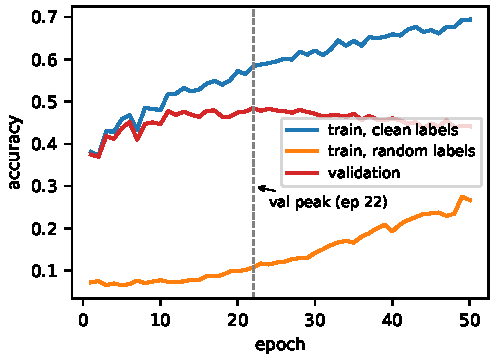
\includegraphics[width=\linewidth]{../figures/q1b_memorisation.pdf}
\caption{Q1b memorisation trajectory. The model fits clean labels first; random labels are only slowly absorbed, and validation peaks (epoch 22) well before the run ends.}
\label{fig:q1b}
\end{figure}

Figure~\ref{fig:q1b} shows clean-subset accuracy rising to 69.4\% by epoch 50 while wrong-label accuracy stays far lower (26.7\%; chance is 10\%).
Useful structure is learned first: validation accuracy peaks at 48.5\% at epoch 22 and then decays to 44.1\% while total train accuracy keeps climbing, which is the classic signature of memorisation starting after generalisable structure is in place.
Even at epoch 50 the noisy subset is far from memorised, so under this budget memorisation pressure shows up as validation decay rather than full fitting of the random labels.

\section{Q2: CNN versus MLP}
\subsection{Fair comparison (Q2a)}
The fairness criterion was fixed before looking at results: same split, same optimiser, learning rate, batch size, epochs, seed, and a parameter budget matched to within 1\%.
CNN: two conv layers (32 and 64 filters, $3{\times}3$, ReLU, max-pool) then a 760-unit FC layer, 1.78M parameters; MLP-L has 1.79M.
Both consume the same raw pixel values.

The CNN reaches 69.9\% test accuracy against 52.5\% for MLP-L (Fig.~\ref{fig:q2a}).
We propose one specific reason, tested next: \emph{weight sharing gives every position the same local filters}, so a filter learned on one part of the image applies everywhere, while the MLP must learn each position's weights separately from the same number of examples.

\begin{table}[t]
\centering\small
\begin{tabular}{lcccc}
\toprule
Model & Params & Clean & Permuted & Gray \\
\midrule
MLP-L & 1.79M & 52.5 & 51.3 & --- \\
CNN & 1.78M & \textbf{69.9} & 46.6 & 60.9$^{\dagger}$ \\
CNN, gray retrain & 1.78M & --- & --- & 63.0 \\
\bottomrule
\end{tabular}
\caption{Q2 compared models, parameter counts, and test accuracy (\%) under the three conditions: natural order, fixed pixel permutation, grayscale. $\dagger$: the RGB-trained CNN evaluated on grayscale test images, without retraining.}
\label{tab:q2sum}
\end{table}

\begin{figure}[t]
\centering
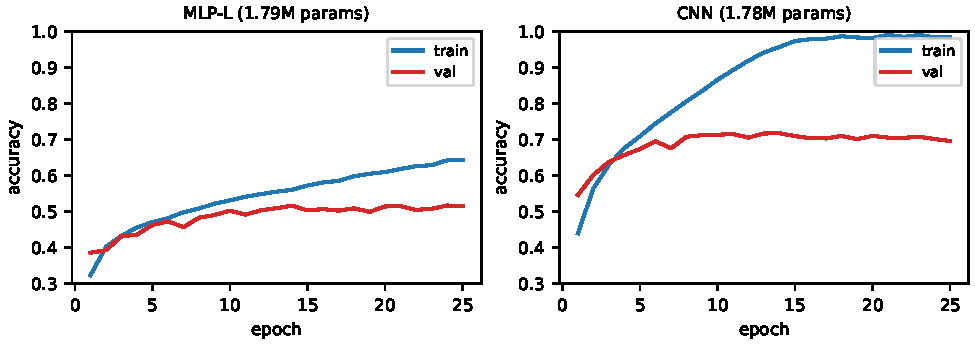
\includegraphics[width=\linewidth]{../figures/q2a_curves.pdf}
\caption{Q2a: CNN and MLP-L under the matched budget. The CNN fits the training set almost perfectly while the MLP is still at 64\%.}
\label{fig:q2a}
\end{figure}

\subsection{Pixel permutation (Q2b)}
CIFAR-10 is modified by one fixed random permutation of the 3{,}072 pixel positions (seed 260008+999, saved to \texttt{split/pixel\_permutation.npy}), applied identically to train, validation and test images.
All pixel values remain available; only their spatial arrangement is destroyed.

Stated in advance: the CNN should lose far more than the MLP, because permutation destroys exactly what weight sharing exploits, while the MLP never depended on adjacency.
Observed (Fig.~\ref{fig:q2b}, Table~\ref{tab:q2sum}): MLP 52.5 $\to$ 51.3 ($-1.2$), CNN 69.9 $\to$ 46.6 ($-23.3$).
The MLP is even slightly insensitive by construction --- permuting inputs only renames its units.
The 23-point collapse of the CNN confirms that its advantage came from local spatial structure, not from extra capacity or tuning: with locality removed the CNN falls below the MLP.

\begin{figure}[t]
\centering
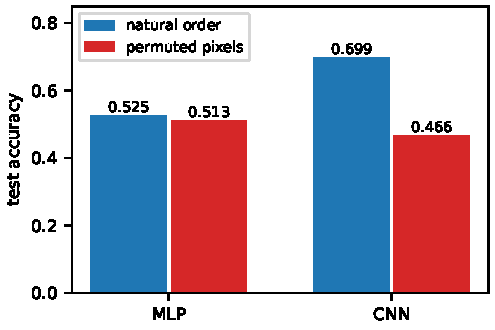
\includegraphics[width=\linewidth]{../figures/q2b_permutation.pdf}
\caption{Q2b: test accuracy before and after the fixed pixel permutation.}
\label{fig:q2b}
\end{figure}

\subsection{Third condition: colour (Q2c)}
Two explanations remain for the CNN's behaviour: it uses colour, or it uses learned spatial filters regardless of channels.
We distinguish them by retraining the identical CNN on grayscale images (mean over channels, same transform applied to the corresponding test images, as required), and additionally evaluating the RGB-trained CNN on grayscale test images.
Errors and confidence are analysed on the test set (Table~\ref{tab:q2c}).

\begin{table}[t]
\centering\small
\begin{tabular}{lcccc}
\toprule
Condition & Acc. & Conf. correct & Conf. wrong & Hi-conf.\ wrong \\
\midrule
RGB CNN, RGB & 69.9 & 0.956 & 0.845 & 16.5\% \\
RGB CNN, gray & 60.9 & 0.936 & 0.828 & 19.9\% \\
Gray CNN, gray & 63.0 & 0.937 & 0.814 & 17.2\% \\
\bottomrule
\end{tabular}
\caption{Q2c test-set error and confidence analysis. ``Hi-conf.\ wrong'' is the fraction of test images with max softmax $>0.9$ that are misclassified.}
\label{tab:q2c}
\end{table}

\begin{figure}[t]
\centering
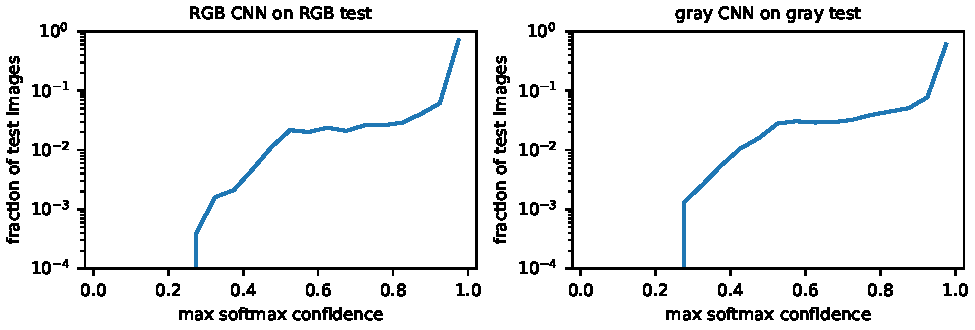
\includegraphics[width=\linewidth]{../figures/q2c_confidence.pdf}
\caption{Q2c max-softmax histograms (log scale). Both models stay saturated near 1 even on wrong predictions.}
\label{fig:q2cconf}
\end{figure}

\begin{figure}[t]
\centering
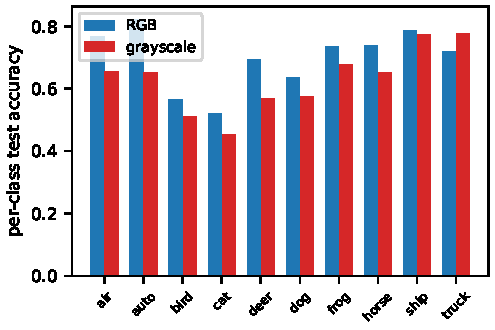
\includegraphics[width=\linewidth]{../figures/q2c_perclass.pdf}
\caption{Q2c per-class test accuracy of the RGB and the grayscale CNN.}
\label{fig:q2cpc}
\end{figure}

Retraining on grayscale recovers 2.1 of the 9.0 points lost when the RGB CNN receives grayscale input (Table~\ref{tab:q2sum}: 60.9 $\to$ 63.0); 6.9 points below the RGB ceiling remain, so colour is worth part of the gap but not most of it.
Per class (Fig.~\ref{fig:q2cpc}), colour helps most for \emph{airplane} (76.7 $\to$ 65.4) and \emph{automobile} (82.3 $\to$ 65.3), consistent with sky/sea backgrounds and painted metal, while \emph{truck} actually improves in grayscale (71.9 $\to$ 77.8).
Confidence stays badly calibrated in all conditions (Fig.~\ref{fig:q2cconf}): mean confidence on wrong predictions is 0.81--0.85, and 16.5--19.9\% of all test images are wrong with $>$0.9 confidence.
Grayscale input shifts mass away from the saturated bin but does not fix calibration.
Linking the three experiments: the CNN's advantage is mostly shared local filtering (Q2b), colour contributes a smaller, class-dependent part (Q2c), and overconfidence persists across all conditions.

\section{Q3: autoencoders}
\subsection{Bottleneck selection (Q3a)}
Three convolutional autoencoders differ \emph{only} in bottleneck channels $c \in \{4, 32, 128\}$ on a $4{\times}4$ grid, i.e.\ 64, 512 and 2048 latent units.
The encoder uses stride-2 convolutions ($3{\to}32{\to}64{\to}64{\to}c$), the decoder mirrors it with transposed convolutions and a sigmoid output; training (Adam $10^{-3}$, 25 epochs, batch 128, MSE loss on $[0,1]$ images) is identical.
Parameter counts grow only from 113k to 129k, so capacity is deliberately held close while the code size spans a factor 32.

\begin{table}[t]
\centering\small
\begin{tabular}{lcccc}
\toprule
$c$ & Units & Params & Val MSE & Test MSE \\
\midrule
4 & 64 & 113{,}159 & 0.009633 & 0.009570 \\
32 & 512 & 116{,}771 & 0.002373 & 0.002361 \\
128 & 2048 & 129{,}155 & \textbf{0.001980} & \textbf{0.001967} \\
\bottomrule
\end{tabular}
\caption{Q3a reconstruction MSE per pixel after 25 epochs. The validation set selects $c{=}128$.}
\label{tab:q3a}
\end{table}

Validation MSE selects $c{=}128$ (Table~\ref{tab:q3a}, Fig.~\ref{fig:q3a}).
The choice is justified by the shape of the gain: going from 64 to 512 units lowers MSE by $7.3 \times 10^{-3}$, while 512 to 2048 adds only $0.4 \times 10^{-3}$.
The code is heavily redundant already at $c{=}32$; we keep $c{=}128$ because it is best on the selection criterion, and note the flattening as the more interesting observation.

\begin{figure}[t]
\centering
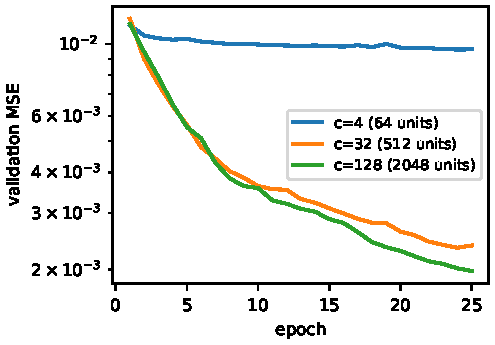
\includegraphics[width=\linewidth]{../figures/q3a_val_mse.pdf}
\caption{Q3a validation MSE during training (log scale).}
\label{fig:q3a}
\end{figure}

\subsection{Where reconstruction helps (Q3b)}
Corruption: additive Gaussian noise, $\sigma{=}0.25$ per pixel on the $[0,1]$ image, clipped to range --- strong enough to shred structure (Fig.~\ref{fig:q3rec}) but the class is still usually inferable by a human.
The DAE has the $c{=}128$ architecture and is trained on corrupted inputs with clean targets, no labels.
A fixed noisy validation/test pair (seeds 777001/888001) is created once so every model is scored on the same corruption.
Classification always uses the \emph{same frozen CNN from Q2a}; nothing is retrained.

\begin{table}[t]
\centering\small
\begin{tabular}{lcc}
\toprule
Input to CNN & Test acc. & MSE vs.\ clean \\
\midrule
Clean images & 69.9 & --- \\
Corrupted & 31.4 & 0.0484 \\
Clean AE recon. & 49.4 & 0.0102 \\
DAE recon. & \textbf{50.9} & \textbf{0.0060} \\
\bottomrule
\end{tabular}
\caption{Q3b: classification of corrupted test images and of their reconstructions.}
\label{tab:q3b}
\end{table}

\begin{figure}[t]
\centering
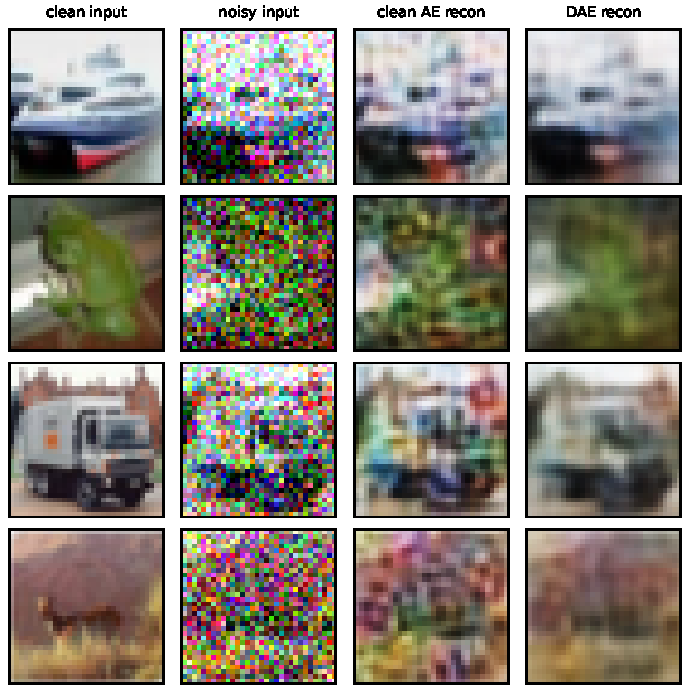
\includegraphics[width=\linewidth]{../figures/q3b_recon.pdf}
\caption{Q3b reconstructions of noisy test images. The clean AE reproduces part of the noise; the DAE output is smoother and loses more detail.}
\label{fig:q3rec}
\end{figure}

Denoising recovers a large part of what the classifier needs: 31.4\% $\to$ 50.9\% (+19.6 points), and the DAE also reconstructs better (MSE 0.0060 vs.\ 0.0102).
It does not recover everything: 19.0 points below the clean-input ceiling remain, and the reconstructions in Fig.~\ref{fig:q3rec} are visibly smoother than the originals, losing exactly the high-frequency detail a CNN filter bank feeds on.
The clean AE, which has never seen noise, already helps (+18.0 points) because the encoder itself is a low-pass map --- but it passes noticeably more residual noise into the classifier.

\subsection{Probes versus reconstruction quality (Q3c)}
Class information is measured without fine-tuning: standardise each encoder's bottleneck, fit logistic regression (max 1000 iterations) on the 45{,}000 training codes, score the test codes.

\begin{table}[t]
\centering\small
\begin{tabular}{lcccc}
\toprule
Encoder & Dim & Probe train & Probe test & Test MSE \\
\midrule
AE $c{=}4$ & 64 & 36.8 & 36.4 & 0.009570 \\
AE $c{=}32$ & 512 & 45.7 & 42.7 & 0.002361 \\
AE $c{=}128$ & 2048 & 49.3 & 44.1 & \textbf{0.001967} \\
DAE $c{=}128$ & 2048 & 53.3 & \textbf{48.0} & 0.004231 \\
\bottomrule
\end{tabular}
\caption{Q3c: linear probe accuracy on frozen codes versus reconstruction quality (MSE on clean test images).}
\label{tab:q3c}
\end{table}

Within the clean-AE family the two quantities \emph{agree}: more capacity gives better reconstruction and better probes in the same order ($c4 < c32 < c128$ in MSE, 36.4 $<$ 42.7 $<$ 44.1 in probe accuracy).
Across training objectives they \emph{disagree}: the DAE reconstructs clean images clearly worse than AE-$c128$ (0.0042 vs.\ 0.0020) yet its codes carry 3.9 points more class information (48.0 vs.\ 44.1).
Removing noise from the training signal buys class-relevant structure at the cost of pixel fidelity, so reconstruction error alone would have ranked the encoders in the wrong order for classification.

\section{Q4 (bonus): SVM and clustering on a frozen representation}
\subsection{C and kernel sweep (Q4a)}
Representation: the encoder of the selected $c{=}128$ autoencoder (2048-d codes), frozen.
Before any model selection we fixed a stratified subset of 10{,}000 training codes (1{,}000 per class, seed 260008, stored in \texttt{data/q4\_fixed.npz} with the StandardScaler fitted on it) and used it for \emph{every} SVM comparison below; validation (5{,}000) and test (10{,}000) are scored through the same scaler.
We sweep $C \in \{0.01, 0.1, 1, 10, 100, 1000\}$ (five orders of magnitude) for three kernels: RBF, polynomial degree 3 with $c_0{=}1$, and linear.
RBF and polynomial are libsvm SVC; the linear kernel solves the one-vs-rest squared-hinge primal $\tfrac12\|W\|^2 + C\sum_{i,c}\max(0,1-y_{ic}f_c(x_i))^2$ with L-BFGS, because liblinear's dual hinge solver did not converge within our compute budget at large $C$; for it we report the fraction of training points with functional margin $\le 1$ as the SV fraction.

\begin{table}[t]
\centering\small
\setlength{\tabcolsep}{3.6pt}
\begin{tabular}{llcccccc}
\toprule
Kernel & Metric & \multicolumn{6}{c}{$C$} \\
 & & 0.01 & 0.1 & 1 & 10 & 100 & 1000 \\
\midrule
\multirow{3}{*}{linear}
 & train & 52.6 & 54.0 & 54.2 & 54.1 & 54.1 & 54.1 \\
 & val & 39.7 & 39.7 & 39.7 & 39.8 & 39.8 & 40.0 \\
 & SV frac. & 1.00 & 1.00 & 1.00 & 1.00 & 1.00 & 1.00 \\
\midrule
\multirow{3}{*}{rbf}
 & train & 31.8 & 41.4 & 71.9 & \textbf{98.7} & 100 & 100 \\
 & val & 30.5 & 37.6 & 47.7 & \textbf{48.6} & 47.8 & 47.8 \\
 & SV frac. & 1.00 & 0.98 & 0.95 & \textbf{0.96} & 0.96 & 0.96 \\
\midrule
\multirow{3}{*}{poly}
 & train & 18.2 & 33.1 & 69.4 & 94.6 & 99.8 & 100 \\
 & val & 16.6 & 26.0 & 37.2 & \textbf{41.8} & 41.1 & 40.0 \\
 & SV frac. & 1.00 & 0.98 & 0.95 & 0.93 & 0.92 & 0.91 \\
\bottomrule
\end{tabular}
\caption{Q4a sweep on the fixed 10{,}000-point subset (train/val accuracy in \%, support-vector fraction). Bold marks the selected setting.}
\label{tab:q4a}
\end{table}

\begin{figure}[t]
\centering
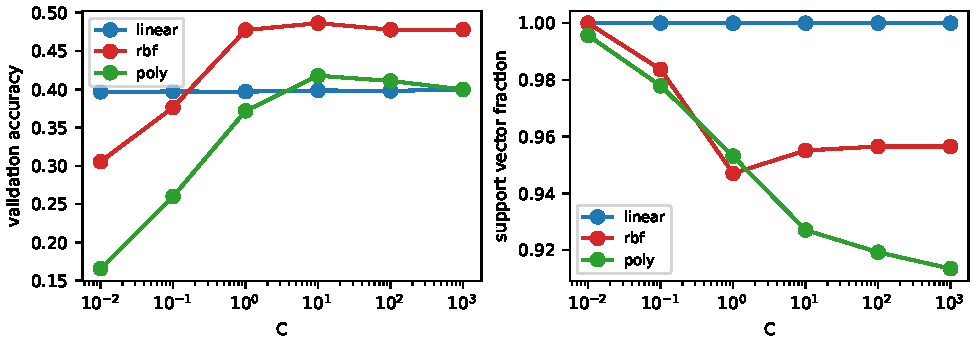
\includegraphics[width=\linewidth]{../figures/q4a_sweep.pdf}
\caption{Q4a: validation accuracy (left) and support-vector fraction (right) versus $C$.}
\label{fig:q4a}
\end{figure}

The sweep shows both regimes the assignment asks for.
RBF: validation climbs from 30.5\% to 48.6\% as $C$ grows to 10 while train accuracy rises 31.8\% $\to$ 98.7\%; beyond $C{=}10$ train hits 100\% and validation \emph{falls} to 47.8\% --- classic overfitting, visible without the test set.
Polynomial behaves the same with a lower ceiling.
Linear is flat: train accuracy stays near 54\% and validation near 40\% at every $C$, and every training point violates the margin, so the representation is far from linearly separable and more capacity cannot fix it --- underfitting at all $C$.
Validation selects RBF with $C{=}10$, which scores 49.8\% on the official test set in a single evaluation (train 98.7\%, SV fraction 0.96).
The 49-point gap between train and test accuracy is the honest cost of the tight AE codes: the SVM can memorise the 10k subset but the codes do not linearly separate the classes.

\subsection{Hard pairs and boundary examples (Q4b)}
From the test confusion matrix of the selected SVM we take the three class pairs with the largest symmetric confusion mass and fit a binary RBF SVM ($C{=}10$) on the pair's training subset.

\begin{table}[t]
\centering\small
\begin{tabular}{lccccc}
\toprule
Pair & Conf.\ mass & Pair acc. & SVs & SV frac. \\
\midrule
cat / dog & 405 & 61.8\% & 1828 & 0.91 \\
automobile / truck & 343 & 75.9\% & 1652 & 0.83 \\
bird / deer & 285 & 67.8\% & 1684 & 0.84 \\
\bottomrule
\end{tabular}
\caption{Q4b: three hardest pairs for the selected SVM, with their binary SVMs trained on the 10k-subset pair samples.}
\label{tab:q4b}
\end{table}

\begin{figure}[t]
\centering
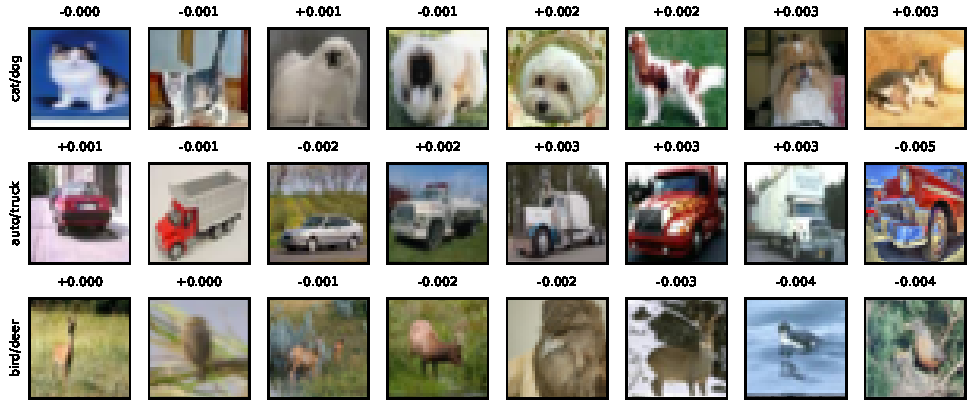
\includegraphics[width=\linewidth]{../figures/q4b_boundary.pdf}
\caption{Q4b: test examples closest to each pair's decision boundary with signed decision scores.}
\label{fig:q4b}
\end{figure}

The SV fractions (0.83--0.91) are lower than the full 10-class problem's 0.96 but still very high: in the AE code space even two classes are barely separated, so a binary boundary needs most samples as support vectors.
The examples nearest the boundary (Fig.~\ref{fig:q4b}) are mostly correctly classified (16 of 24), and their scores are tiny ($|f| \le 0.005$).
Visually they are the expected failures: poses where cat and dog silhouettes coincide, trucks that share the box shape and colour of cars, deer and birds in grass.
The pattern matches the geometry of the representation: reconstruction-driven codes preserve coarse shape and colour mass but discard the fine parts (ears, wheels, beak) that separate these pairs, which is exactly why the same pairs dominate the 10-class confusion.

\subsection{Clustering versus classification (Q4c)}
$k$-means is fitted on the same scaled 10{,}000 training codes without labels; $k \in \{10,20,30,40\}$ is chosen by validation-set silhouette, which selects $k{=}10$ (0.036 vs.\ $\le 0.008$ for all others --- the representation has weak cluster structure overall).
Test labels are used only after assignment.

\begin{table}[t]
\centering\small
\begin{tabular}{lc}
\toprule
Metric (test set) & Value \\
\midrule
ARI (clusters vs.\ classes) & 0.042 \\
NMI & 0.086 \\
Cluster purity & 22.6\% \\
ARI (clusters vs.\ SVM predictions) & 0.061 \\
NMI (clusters vs.\ SVM predictions) & 0.122 \\
SVM test accuracy & 49.8\% \\
\bottomrule
\end{tabular}
\caption{Q4c: clustering quality and its disagreement with the SVM.}
\label{tab:q4c}
\end{table}

\begin{figure}[t]
\centering
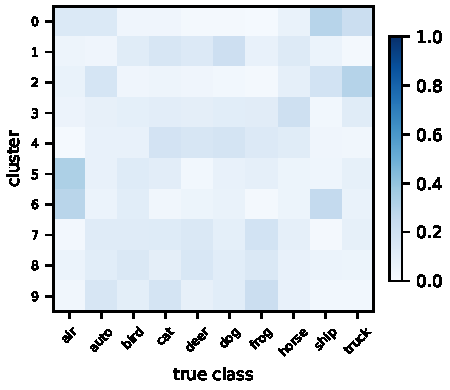
\includegraphics[width=0.9\linewidth]{../figures/q4c_contingency.pdf}
\caption{Q4c: cluster-to-class contingency (row-normalised), $k{=}10$.}
\label{fig:q4c}
\end{figure}

The contrast with the SVM is stark: purity 22.6\% and ARI 0.042 against 49.8\% supervised accuracy.
Clusters and predictions barely agree with each other either (ARI 0.061, NMI 0.122).
The contingency table (Fig.~\ref{fig:q4c}) shows where the two disagree most: cluster 8 absorbs parts of five classes (bird, cat, deer, dog, frog each 19--31\%), so a whole animal super-group that the SVM still splits into separate classes is one unsupervised cluster; conversely \emph{automobile} (SVM 63.1\%) has no dominant cluster of its own (21.6\% in cluster 8), and \emph{truck} lands mainly in cluster 2 (30.8\%) with no strong second home.
Classification and clustering therefore lead to different conclusions about the same representation: the code space groups images by coarse appearance (background, silhouette size), not by the class boundaries the SVM is trained to draw.

\section{Reproduction}
Every reported number is produced by the committed scripts in this order:
\texttt{split\_data.py}, \texttt{q1a\_train\_mlps.py --model \{mlpL,mlpB,mlpS,mlpP\}}, \texttt{q1b\_memorisation.py}, \texttt{q2a\_train\_cnn.py}, \texttt{q2b\_permutation.py --model \{mlpPerm,cnnPerm\}}, \texttt{q2c\_train\_gray.py}, \texttt{q2c\_analysis.py}, \texttt{q3a\_autoencoders.py --bottleneck \{4,32,128\}}, \texttt{q3b\_train\_dae.py}, \texttt{q3b\_eval.py}, \texttt{extract\_features.py --run \{...\}}, \texttt{q3c\_probes.py}, \texttt{q4\_prepare.py}, \texttt{q4a\_svm\_sweep.py}, \texttt{q4b\_pairs.py}, \texttt{q4c\_clustering.py}, \texttt{make\_figures.py}.
All runs are seeded; on a fixed thread count the whole pipeline reruns to the same numbers. The environment is pinned in \texttt{requirements.txt}.

{\small
\begin{thebibliography}{9}
\bibitem{krizhevsky2009} A.~Krizhevsky. Learning Multiple Layers of Features from Tiny Images. Technical report, University of Toronto, 2009.
\bibitem{vincent2008} P.~Vincent, H.~Larochelle, Y.~Bengio, P.-A. Manzagol. Extracting and Composing Robust Features with Denoising Autoencoders. ICML, 2008.
\bibitem{cortes1995} C.~Cortes, V.~Vapnik. Support-Vector Networks. Machine Learning 20(3):273--297, 1995.
\bibitem{macqueen1967} J.~MacQueen. Some Methods for Classification and Analysis of Multivariate Observations. Berkeley Symposium on Mathematical Statistics and Probability, 1967.
\end{thebibliography}
}

\end{document}
